\subsection{L'interface cliente avec Angular}
\label{subsec:frontend-angular}

\paragraph{}
Les sites web se complexifient d'année en année.
Pour faire face à l'exigence croissante des besoins en interface utilisateur, il est indispensable d'utiliser un \gls{g-framework} adapté aux enjeux d'aujourd'hui.
J'ai choisi d'utiliser \Gls{g-angular}.

Ce projet propose de structurer le code en différentes sortes de structures et les transforme en fichiers compréhensibles par un navigateur internet.
Au final, le navigateur ne recevra que des fichiers \gls{a-html}, des fichiers \gls{a-css}, des fichiers \gls{g-javascript} et des fichiers médias comme des images ou des sons par exemple.

\begin{figure}[ht]
    \centering
    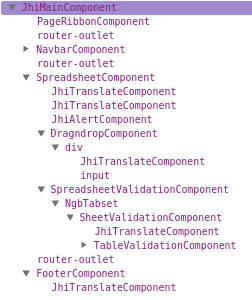
\includegraphics[width=0.5\textwidth]{images/diagrams/angular-components.png}
    \caption{Le découpage des composants visibles sur la page de gestion des classeurs Excel}
    \label{fig:angular-components}
\end{figure}

\begin{figure}[ht]
    \centering
    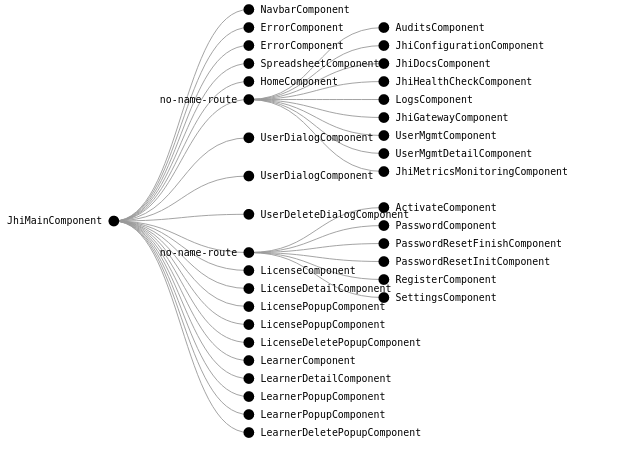
\includegraphics[width=0.8\textwidth]{images/diagrams/angular-routes.png}
    \caption{Les composants sont organisés selon les routes qui y mènent}
    \label{fig:angular-routes}
\end{figure}

\paragraph{}
l'application tire particulièrement profit du découpage afin de proposer des composants utilisables dans tous les contextes (la figure \ref{fig:angular-components} et la figure \ref{fig:angular-routes} montrent un exemple).

Par exemple, pour la réception des fichiers, j'ai mis en place un composant prêt à l'emploi et une directive à appliquer sur un composant existant (\lstinline{DragndropComponent} sur la figure \ref{fig:angular-components}).
Cette directive est une possibilité d'\Gls{g-angular} permettant d'associer un comportement et des fonctionnalités à d'autres composants.
J'ai prévu celle-ci en vue des développeurs qui voudraient créer leur propre élément graphique.

L'annexe \ref{ch:angular-components} parcourt le code de ces composants.

\paragraph{}
J'ai implémenté la gestion des évènements en utilisant la bibliothèque RxJS.
C'est une des librairies les plus populaires dans le monde web ces jours-ci et ses fonctionnalités ont été implémentées dans de nombreux langages.
Elle permet de réagir aux évènements de différentes façons.

\paragraph{}
Le respect de l'authentification est géré par un système de garde.
Les pages de l'application requérant un accès spécial sont protégées sur base de leur chemin.
Le garde s'active dès que l'on navigue vers une route qu'il protège, peu importe le chemin emprunté. 

\paragraph{}
Pour styliser mon application, j'ai utilisé la bibliothèque Boostrap en version 3.
Elle permet de rapidement créer des pages web belles et cohérentes avec un code léger et structuré.

\paragraph{}
Pour les différentes icônes utilisées sur le site, j'ai utilisé la librairie d'icônes Font Awesome.
